\begin{multicols}{3}[\section{4G/LTE}]

\rhead{Autorin: Yuliya Ukolava}
\lfoot{Letzte Bearbeitung: 17.04.2016}

\newrefsegment

\begin{boxedminipage}{\linewidth}
\begin{tabular}{p{2,1 cm}p{2.7 cm}}
\textbf{Steckbrief}& \\
\end{tabular}
\begin{tabular}{p{2,1 cm}|p{2.7 cm}}
      Einsatz seit & 2009\\
      \hline
      Frequenz"-bereich  & \SI{ 20 }{\mega\hertz}\\
      \hline
      Datenrate & \SI{100}{bit/s}\\
      \hline
      Verbreitung & Weltweit\\
\end{tabular}
\end{boxedminipage}
\par

\subsection*{Überblick}
LTE steht für Long Term Evolution (langfristige Entwicklung) und folgt als vierte Mobilfunkgeneration (4G) auf die vorigen Standards GSM (2G) und UMTS (3G). ~\cite{4GLTE.1}
Es soll besonders schnelle Geschwindigkeiten beim Surfen im mobilen Internet ermöglichen. 


\subsection*{Technische Erläuterungen}
Um den wachsenden Datenverkehr im Mobilfunknetz abwickeln zu können ist eine breitbandige Anbindung der Basisstationen an das Kernnetz erforderlich. Hierfür setzt man bevorzugt Richtfunk und Glasfaser ein. Das Transportnetz, das die Basisstationen mit dem Kernnetz verbindet besteht hauptsächlich aus Routern und Switche, wie sie üblicherweise in der Netzwerktechnik eingesetzt werden. Damit das möglich ist, sind in LTE gängige Netzwerktechniken und -protokolle zusammengeführt. Die Systemarchitektur von GSM und UMTS bestand hauptsächlich noch aus teurer Spezialhardware.

Um die Übertragungskapazität zu erhöhen wird beim Informationsaustausch zwischen Basisstation und dem Kernnetz gespart. Angestrebt wird eine einfache Integration in das bestehende Mobilfunknetz und eine einfache Architektur mit sich selbst konfigurierenden Basisstationen.
Die LTE-Basisstationen sind kleiner als GSM- und UMTS-Basisstationen. So können die Netzbetreiber die LTE-Basisstationen an Orten installieren, die sich für GSM- und UMTS-Basisstationen weniger eignen. Das erlaubt die Funkversorgung von Orten, die sonst nur schwer oder gar nicht zugänglich sind.

Die LTE-Netzarchitektur wird als Evolved Packet System (EPS) bezeichnet. Es wird in das Funkzugangsnetz Evolved UMTS Terrestrial Radio Access Network (EUTRAN) und das Kernnetz Evolved Packet Core (EPC) unterteilt. Das EPC ist vollständig paketorientiert und setzt auf das Internet Protokoll (IP).
\begin{Figure}
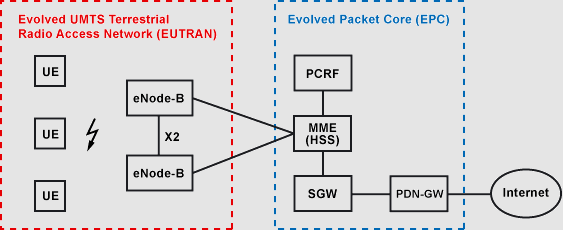
\includegraphics[width=\linewidth]{Kapitel/4GLTE/Grafiken/Modell.png}
\captionof{figure}{EPS - Evolved Packet System~\cite{4GLTE.2}}
\label{fig:vorlage.vorlesungssaal}
\end{Figure}

Im EUTRAN werden die mobilen Endgeräte als User Equipment, kurz LTE UE, bezeichnet. Die Funktion der Basisstationen ist aus der UMTS-Netzarchitektur abgeleitet und tragen deshalb die Bezeichnung eNode-B. In der LTE-Netzarchitektur sind die Basisstationen mit ihren benachbarten Basisstationen und dem Kernnetz verbunden. Die Schnittstelle X2 zwischen den Basisstationen ermöglicht schnelles Handover.
Für die Anmeldung der Teilnehmer am Netz und deren Lokalisierung ist die Management Mobility Entity (MME) zuständig. Die MME greift auf den Home Subscriber Service (HSS) zu. Hat das Endgerät einen gültigen Account wird ihm ein Serving-Gateway (SGW) zugewiesen. Von dort besteht eine Verbindung zum PDN-GW, dass die Verbindung zum Internet herstellt und dem Endgerät eine IP-Adresse zuweist.
Im Kernnetz befindet sich außerdem die PCRF (Policy and Charging Rules Function). Hier werden die Leistungen, die im Tarif festgelegt sind, geregelt. ~\cite{4GLTE.3}

Damit mehrere Mobilfunkgeräte gleichzeitig Daten übertragen können arbeitet LTE mit skalierbaren und individuellen Kanälen. Das bedeutet konkret, dass das Frequenzspektrum geteilt und einzelnen Geräten für eine bestimmte Zeit zugewiesen wird.
Für den Downlink wird OFDMA verwendet. OFDMA teilt das zur Verfügung stehende Frequenzband in viele schmale Bänder (Kanäle) auf. Das bedeutet, dass LTE mit unterschiedlich großen Frequenzbändern auskommen. Die Bandbreite wird flexibel genutzt, um das Äußerste an Übertragungsleistung aus den Frequenzen herauszuholen.

Das Frequenzband (\si{10},\si{15},\SI{20}{\mega\hertz}) wird in Subcarrier zu je \SI{15}{\kilo\hertz} aufgeteilt. Jeweils 12 Subcarrier werden zu einem Ressource-Block (RB) zusammengefasst, was die kleinste Einheit dessen ist, was einem LTE-Gerät zugewiesen werden kann. Ein Gerät kann je Richtung einen bis mehrere Ressource-Blöcke belegen. Die Anzahl hängt von der Auslastung der Zelle und der Signalgüte ab. Die Obergrenze ergibt sich aus der Breite des Frequenzblocks, den die Basisstation verwendet. Bei einem \SI{10}{\mega\hertz}-Frequenzblock sind das 50 Ressource-Blöcke. Bei \SI{20}{\mega\hertz} sind es 100.

Zeitlich ist die Übertragung eines Blocks auf \SI{10}{\milli\second} festgelegt (Frame). Das sind 10 Blöcke pro Sekunde. Jeder Frame besteht wiederum aus 10 Subframes. Pro Subframe lässt sich ein Transport-Block übertragen. Die Größe des Transport-Blocks hängt im wesentlichen von der Signalgüte ab. Die Signalgüte bestimmt, welche Modulation verwendet wird, wie das Verhältnis zwischen Nutzdaten und Fehlerkorrektur (Code-Rate) ist und wie viele Ressource-Blöcke verwendet werden. Dabei hängen diese drei Parameter direkt miteinander zusammen.

Spezielle Algorithmen wählen die geeigneten Kanäle aus und berücksichtigen dabei die Einflüsse aus der Umgebung. Dabei werden nur die Träger zur Übertragung genutzt, die für den Nutzer am günstigsten sind.
Für den Uplink wird SC-FDMA verwendet (Single Carrier Frequency Division Multiple Access). Das ist ein Einträgerzugriffsverfahren und OFDMA sehr ähnlich. SC-FDMA weist geringer Leistungsschwankungen auf und macht einfacher Leistungsverstärker möglich. Das schont vor allem den Akku mobiler Geräte.

LTE arbeitet auch mit räumlich separierte Datenströmen. Die LTE-Spezifikation sieht 4 Antennen in der Basisstation und 2 Antennen in den Endgeräten vor. Das Sendesignal wird zur Übertragung an mehrere Sendeantennen weitergeleitet. Die Empfangssignale werden von zwei Antennen empfangen (MIMO). Aus beiden Signalen wird dann ein besseres Signal herausgerechnet. Damit erreicht man einen besseren Datendurchsatz, weil beide Sende- und Empfangspfade nicht den gleichen Störungen (Verluste und Interferenzen) unterliegen. Dieses Verfahren ist in abgewandelter Form auch in WLANs nach IEEE 802.11n spezifiziert. Zusätzlich verwendet LTE, wie HSPA auch, das gleiche Shared-Channel-Prinzip, sowie HARQ und AMC. ~\cite{4GLTE.4}
 

\subsection*{Einsatz}
„Anytime-anywhere“, also immer und überall mobile Kommunikation betreiben zu können, dafür soll 4G stehen. Primär soll das heißen: ortsunabhängiger drahtloser Breitband-Internetzugang. Multimedia Messaging Service (MMS), Video Chat, High Definition Radio (HD-Radio), mobile TV, High Definition TV content (HDTV), DVB und normales Telefonieren soll in diesem Netz möglich sein.
LTE bietet als rein paketbasiertes Netz keinen separaten, verzögerungsfreien Kanal für Sprachdaten an. Daher können Telefonate im LTE-Netz ausschließlich per Voice over IP übertragen werden. Zum Telefonieren muss sich ein Handy derzeit beim LTE-Netz abmelden und ins 3G- (UMTS) oder 2G-Netz (GSM) wechseln. Bei diesem Circuit Switch Fallback (CSFB) genannten Verfahren entstehen beim Rufaufbau Verzögerungen von einigen Sekunden. ~\cite{4GLTE.5}
Durch die bessere Ausnutzung der Frequenzen ist es möglich, mehr Benutzer gleichzeitig mit Daten zu versorgen, woraus sich ein geringerer Preis pro Datenpaket ergibt. 
Am meisten aber dürften die Bewohner ländlicher Gegenden von der neuen 4G-Technik profitieren: War dort bis jetzt nur sehr langsames oder gar kein DSL möglich, so kann man nun die entsprechenden Orte per Mobilfunk anbinden und so mit schnellen Internet-Zugängen versorgen. ~\cite{4GLTE.6}

\end{multicols}
\newpage
\section*{Historische Entwicklung}
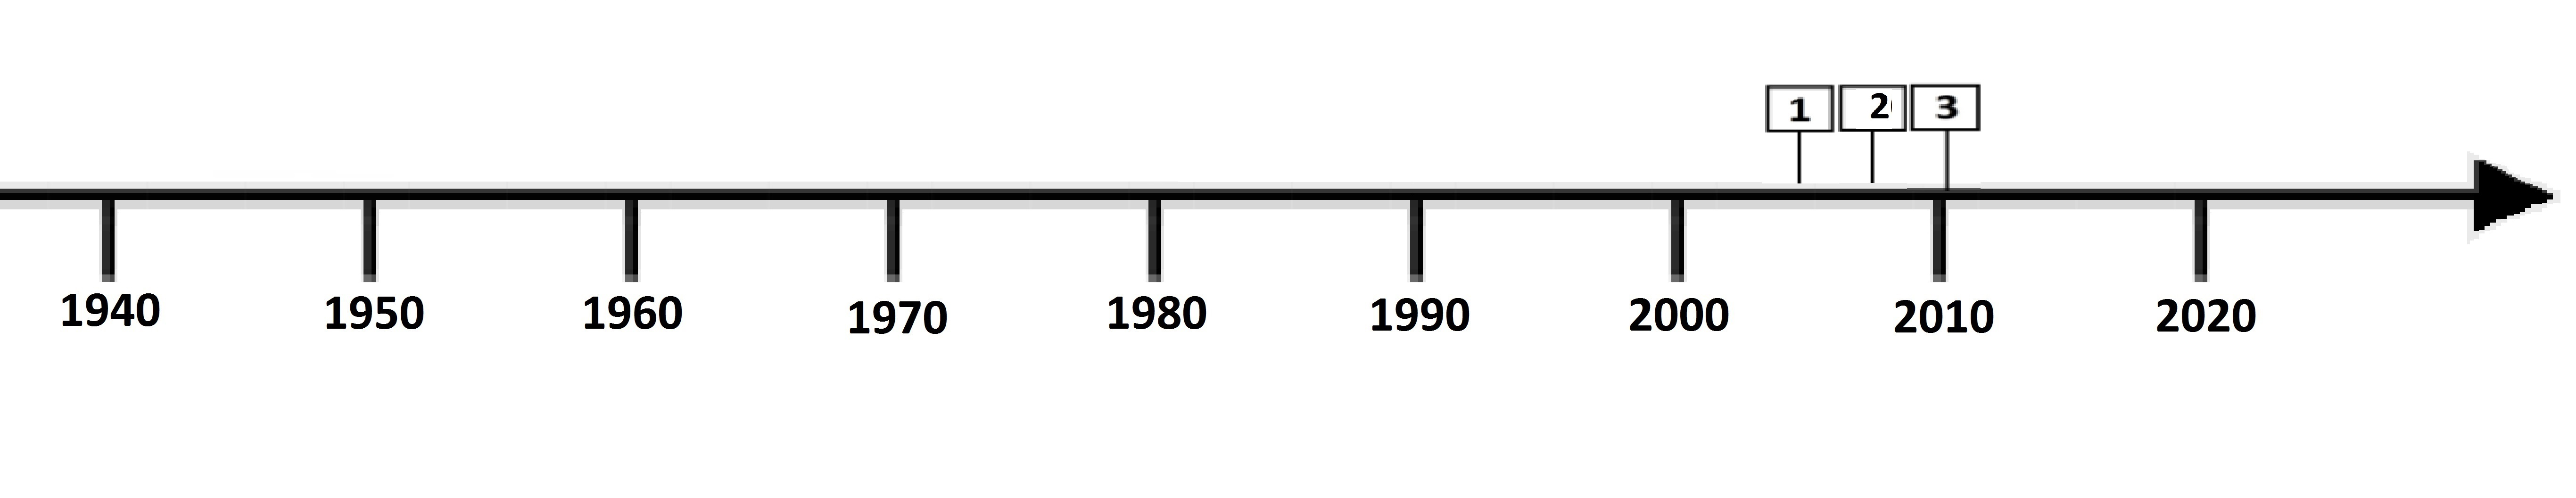
\includegraphics[width=\textwidth]{Kapitel/4GLTE/Grafiken/Zeitstrahl}
\par
\noindent
\begin{tabular}{|p{1 cm}|p{3 cm}|p{13.55 cm}|}
	\hline
	Nummer & Datum & Entwicklungsschritte\\
	\hline
	1 &  September 2006 & Siemens Networks, heute Nokia Solutions and Networks, zusammen mit der Nomor Research GmbH zeigt erstmals einen Emulator eines LTE-Netzwerks mit Live-Applikationen.\\
	\hline
	1 & November 2006 & Die erste LTE-Demonstration in Hongkong in der Öffentlichkeit. \\
	\hline
	2 & 2008 & Auf dem GSMA Mobile World Congress in Barcelona zeigte Ericsson erstmals eine Ende-zu-Ende-Verbindung mit LTE auf kompakten Mobilgeräten. Es wurden Datenraten von \SI{25}{Mbit/s} im Uplink und Downlink demonstriert.\\
	\hline
	2 & Im März 2008 & In einem Feldtest von NTT DoCoMo werden \SI{250}{Mbps} demonstriert.\\
	\hline
	2 &  Ende 2008 &  Es wird von LG ein LTE-Chip vorgeführt, welcher Datenraten von \SI{60}{Mbps} erreicht, was etwa dem Achtfachen der HSDPA-Cat8-Datenrate von \SI{7,2}{Mbps} entspricht.\\
	\hline
	3 & 14. Dezember 2009 & Die ersten kommerziellen LTE-Netzwerke von TeliaSonera werden in Stockholm und Oslo in Betrieb genommen.\\
	\hline
	3 & Mai 2010 & In Deutschland wird LTE mit der Frequenzversteigerung durch die Bundesnetzagentur im  eingeführt.\\
	\hline
\end{tabular}
\par
\begin{multicols}{3}
\subsection*{Anbieter und Gremien} 

Die Deutsche Telekom/T-Mobile, Vodafone, o2 und E-Plus sind die deutschen LTE-Anbieter. Der Düsseldorfer Netzbetreiber E-Plus ist erst im März 2014 mit 4G gestartet. Die beste LTE-Netzabdeckung in Deutschland in der Fläche bieten aktuell die Deutsche Telekom und Vodafone. Diese beiden Anbieter sind auf dem Land (LTE als DSL-Ersatz) und in den Städten stark mit 4G vertreten, während o2 und E-Plus in den Städten eine echte Alternative zu den großen Netzbetreibern sind.
Der 4G-Ausbau der LTE-Anbieter geht in Deutschland seit dem LTE-Start schnell voran. Seit November 2012 haben die deutschen Netzbetreiber ihre Versorgungsverpflichtungen erfüllt und alle Weißen Flecken in den einzelnen Bundesländern geschlossen. Heute beträgt die LTE-Abdeckung deutschlandweit mittlerweile 69 Prozent. Viele deutsche Großstädte bieten dazu eine ausgezeichnete 4G-Netzabdeckung von über 90 Prozent. Nutzer können dort bei einem Anbieter wie T-Mobile oder Vodafone in gut ausgebauten Netzen mit bis zu \SI{150}{Mbit/s} surfen. ~\cite{4GLTE.7}

\subsection*{Ausblick}
Generell zeigt die Prognose, dass der Bedarf an schnellem Internet für unterwegs stetig wächst und auch die Ansprüche der Nutzer an die Mobilfunkanbieter wachsen. Diese Entwicklung geht einher mit immer schneller und besser werdenden Smartphones und Tablets, die unter anderem dafür genutzt werden, Medieninhalte via Streaming mobil auf das jeweilige Gerät zu bringen. Hierbei ist eine leistungsstarke, mobile Datenverbindung natürlich unabdingbar. 4G gibt viele Möglichkeit im Bereich mobiler Datenübertragung und durch steigende 4G-Netzabdeckung und Einführung von LTE als „echten“ DSL-Ersatz soll dieser Bedarf abgedeckt werden. Aber es gibt immer noch viel Potenzial und Erweiterungsoptionen. Deswegen wird es inzwischen bereits am 4G-Nachfolger 5G gearbeitet. 


\printbibliography[segment=14,heading=subbibliography]
\end{multicols}


\newpage